\chapter{Results and Discussion} 
\label{chp:results}
In this chapter, we present the results of the experiments described in Chapter~\ref{chp:experiments} and discuss the performance of the models.
First, in Section~\ref{sec:test-data-results}, we describe the development, training and testing split of the dataset.
Then, we present the results of the graph combination model and discuss the most important features of the logistic regression classifier.
Moreover, we compare it to the performance of the iterative models in the same test dataset and explain the shortcoming of the graph combination model.
Second, we display the results of the iterative models using the entire \wikirfa dataset in Section~\ref{sec:complete-reults}.
Further, we examine the performance of the iterative models and discuss the optimal selection of threshold to predict results.
Lastly, the results of the voting order experiments are presented in Section~\ref{sec:voting-order-results}.
We analyse the significance of the voting order on the performance of the iterative models.


\section{Test Dataset Results}
\label{sec:test-data-results}
As we describes in Section~\ref{subsec:data-prep}, for the graph combination model requires the \wikirfa dataset to be split into three part to prevent data leak.
Although we performed the experiments for many variation of these three splits, we will show the results from the $30-30-40$ split into development (dev), training (train) and testing (test) respectively.
As the model aims to predict votes, we choose to split it on the percentage of votes, as seen in Table~\ref{tab:data-splits}.
We round up the nearest RfA ending so that we have contiguous elections in each split.
In Table~\ref{tab:data-splits}, we see this manifested as small overlaps between the last dates of the previous splits and the first dates.
The time frame overlap is almost exactly seven days, the exact duration a RfA.
Next, we present the details of the auxiliary and signed graphs formed from the dev dataset and the graph combination model's performance on the test dataset.

\begin{table}[htp]
    \centering
    \caption{\wikirfa dataset split information}
    \label{tab:data-splits}
    \begin{tabular}{lcccc}
        \toprule
        Feature & Development & Training & Testing \\
        \midrule

        Percentage &30\% & 30\% & 40\% \\
        Number of votes & 62833 & 62807 & 83830 \\
        Number of RfAs &1668& 1551&1314 \\
        First Date &22/02/2004 & 31/10/2006 &24/06/2008 \\
        Last Date &06/11/2006& 30/06/2008 & 01/01/2019
        \\  
        

        \bottomrule
        \end{tabular}
\end{table}

Next, we also show the results of the iterative models on the test dataset.
We achieve this by evaluating the iterative models' results in the same time period as the test data.
Through this approach, we can compare the benefits of the iterative model, which can utilize both the development and training datasets to learn and update its respective relationship graph.

We provide the evaluation metrics for all models along with the baseline for the test dataset, as seen in Table~\ref{tab:test-results}.
The \aucnegPR baseline shows that negative votes are the minority in the test test.
Similarly, the \aucposPR baseline shows that a model predicting all votes as support votes can achieve nearly $77\%$ accuracy.
Now, we discuss the results of each model in more detail.


\begin{table}[htp]
    \centering
    \caption{Results of different models for the test split of the \wikirfa dataset}
    \label{tab:test-results}
    \begin{tabular}{lccc}
        \toprule
        Model & AUC-ROC & \aucposPR  & \aucnegPR \\ 
        \midrule
        
        Baseline & 0.5 & 0.776 & 0.224 \\

        Graph Combination &  0.542 & 0.798 & 0.251 \\

        Iterative Balance &  0.815 & 0.922 & 0.614 \\

        Iterative Status & 0.754 & 0.9 & 0.486 \\
        
        \bottomrule
        \end{tabular}
\end{table}

\subsection{Graph Combination Model Results}
We start by describing the details of the auxiliary and signed graphs formed from the dev dataset, as seen in Table~\ref{tab:test-graphs}.
The \textit{\% of test users covered} refers the percentage of unique users in the test dataset present in the graph. 
It can be used as a proxy to measure the amount of information a graph can provide to a vote in a RfA in the test dataset.
We see that the \textit{similarity graph} is fairly dense and is completely connected, as we chose the minimum similarity of an edge of $0.03$ to be considered viable.
It also has the largest coverage of nodes in the test dataset.
The \textit{talk graph} also has a large strongly connected component (as it is directed) and a smaller test user coverage.
The \textit{social interaction graph} is the same as the talk graph, but is unweighted, therefore, has the same statistics as the talk graph.
As we explained in Section~\ref{subsec:talk-interaction-graph}, we also include the reversed talk and social interaction graphs to gain additional features.
The \textit{signed graph} by far is the smallest, lest dense and weakest connected graph of all the graphs.
This is because, the signed graph only contains the voting data from the dev dataset.
It will contribute the triadic feature and is hence fine for that task.

\begin{table}[htp]
    \centering
    \caption{Information of graphs formed using development data split}
    \label{tab:test-graphs}
    \begin{tabular}{lccccc}
        \toprule
        Graph & $|G|$ & $\|G\|$ & density & \shortstack{largest\\  component \\size} & \shortstack{\% of \\test users\\ covered}\\ 
        \midrule
        
        Similarity Graph & 6368 &1463465 & 0.0721 & 6368 & 27.3\\
        
        Talk Graph & 5477 & 213307 & 0.0071 & 3489 & 18.9\\

        Signed Graph & 4675 & 65595 & 0.003 & 1083 & 9\\

        \bottomrule
        \end{tabular}
\end{table}

Using these auxiliary and singed graphs we prepare the training and testing feature matrices $\mathbf{X}$ and $\mathbf{X}_{text}$ and target vectors, $\mathbf{y}$ and $\mathbf{y}_{test}$ respectively.
We train the \textit{Logisitc Regression} model on the train feature matrix and targe vector using cross validation.
The feature importances of the trained LR model are shown in Figure~\ref{fig:lr-feature-importances}.
We see both, the five auxiliary features and the 36 triadic features.
\textit{Talk Graph R} and \textit{Social Interactions R} features refer to the reversed version of the talk and social interaction graphs respectively.
We see that the topic similarity graph has the largest coefficient.
The importance of the similarity feature amongst the auxiliary feature can be explained by the fact that, the topic similarity has the largest coverage of test users and therefore contributes the most information.

Among the other features the triad \textit{FB++} has the next largest coefficient.
This result is consistent with balance theory, which would predict a positive edge to maintain the balance in the triad.
However, for this triad, status theory does not have a preference of either a positive or negative edge.
Attempting to interpret the result in terms of status theory we have: if a candidate and voter have a mutual friend who they both respect, then it is more likely that the voter will support the candidate.
Though this motivation is not a typically expected behaviour, it might suggest some unique cognitive biases present in voters. 

The other triadic feature that is significant is the triad "FB-+".
Yet, here the coefficient is negative, indicating that the prediction is more likely to be a negative edge, i.e., an oppose vote.
This result again is consistent only with balance theory.
Balance theory predicts the vote is negative to balance the resulting triad to be balanced.
Status theory implies that, if the candidate and voter share a common friend, who looks up to the candidate, but the voter does not respect, then the voter is ambivalent to the candidate.
However, the result indicate that the voter in this case has a negative view of the candidate and votes against them more often.
Therefore, we see the results agreeing more strongly with balance theory rather than status theory.

And then, we see that both versions of the social interaction graphs are more significant than the talk graph.
This indicates that simple existence correspondence is more important than the amount of correspondence or the direction of correspondence between voters and their voting neighbourhood.

\begin{figure}[htp]
    \centering
    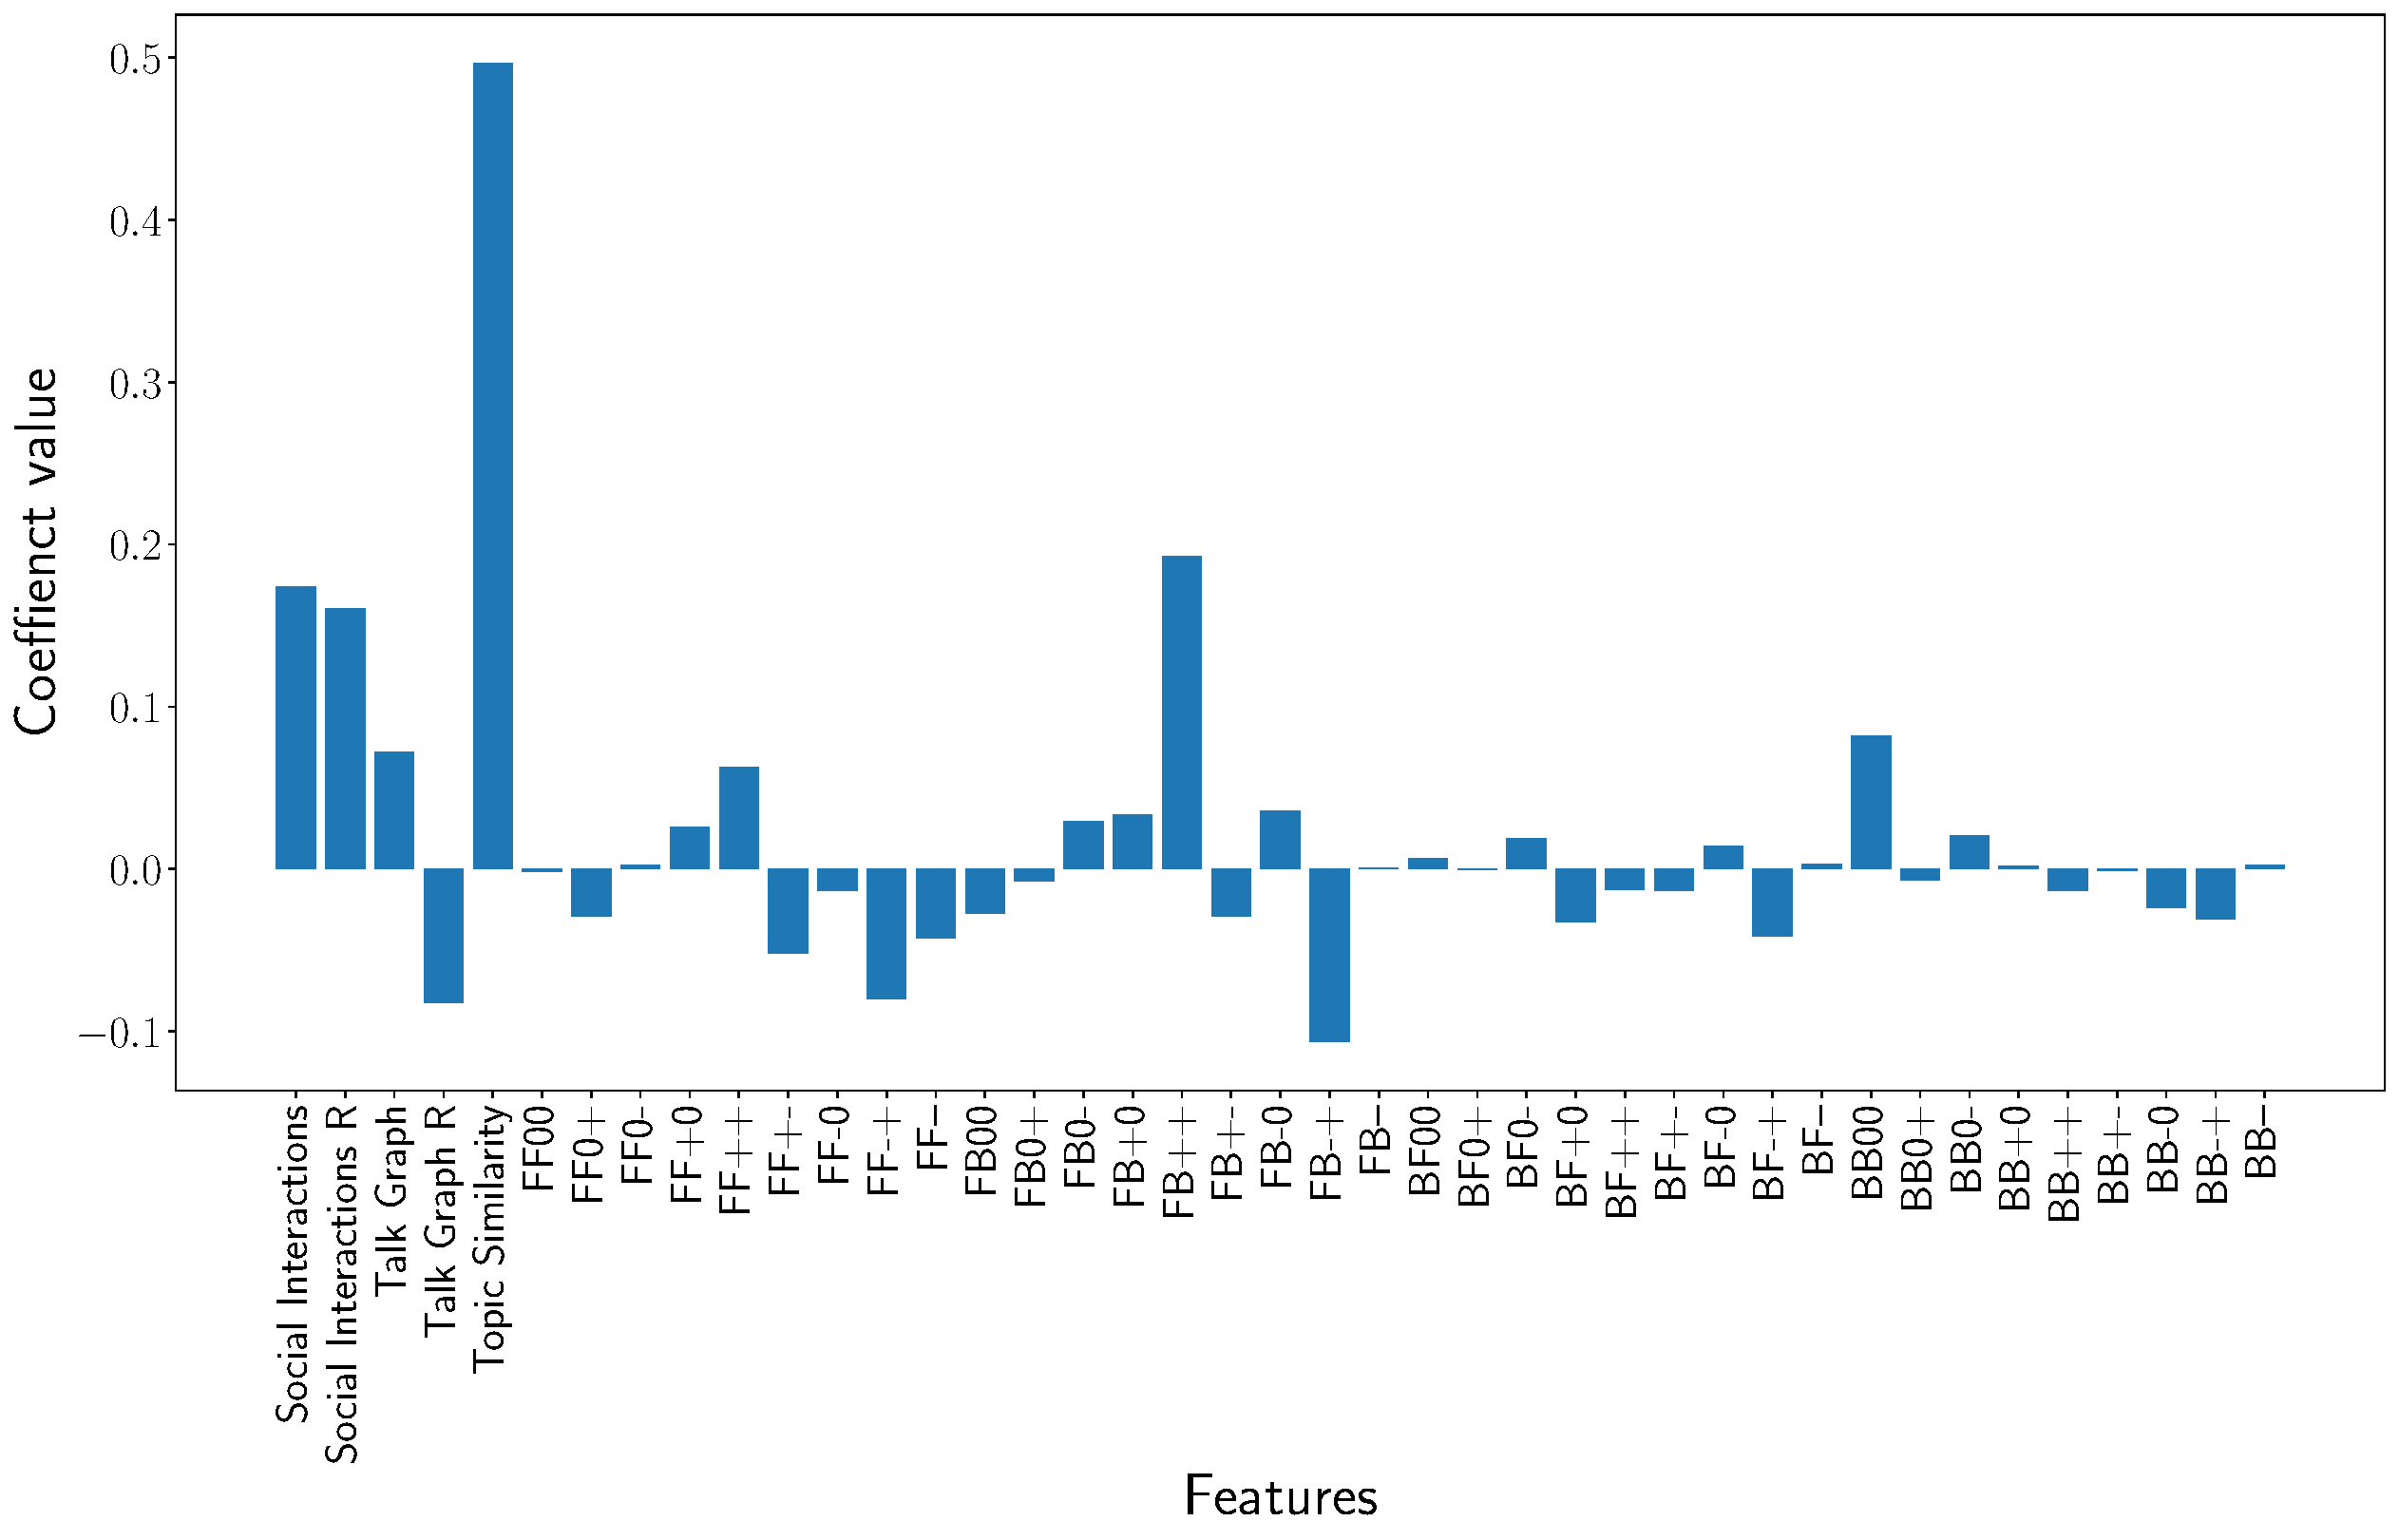
\includegraphics[width=\textwidth]{images/Logistic Regression_features.pdf}
    \caption{Feature importances for Logistic Regression model }
    \label{fig:lr-feature-importances}
\end{figure}


Then, we tested the trained LR model on the test feature matrix and evaluated the output with the target vectors.
The results and the evaluation metrics are seen in Table~\ref{tab:test-results}.

\begin{figure}[htp]
    \centering
    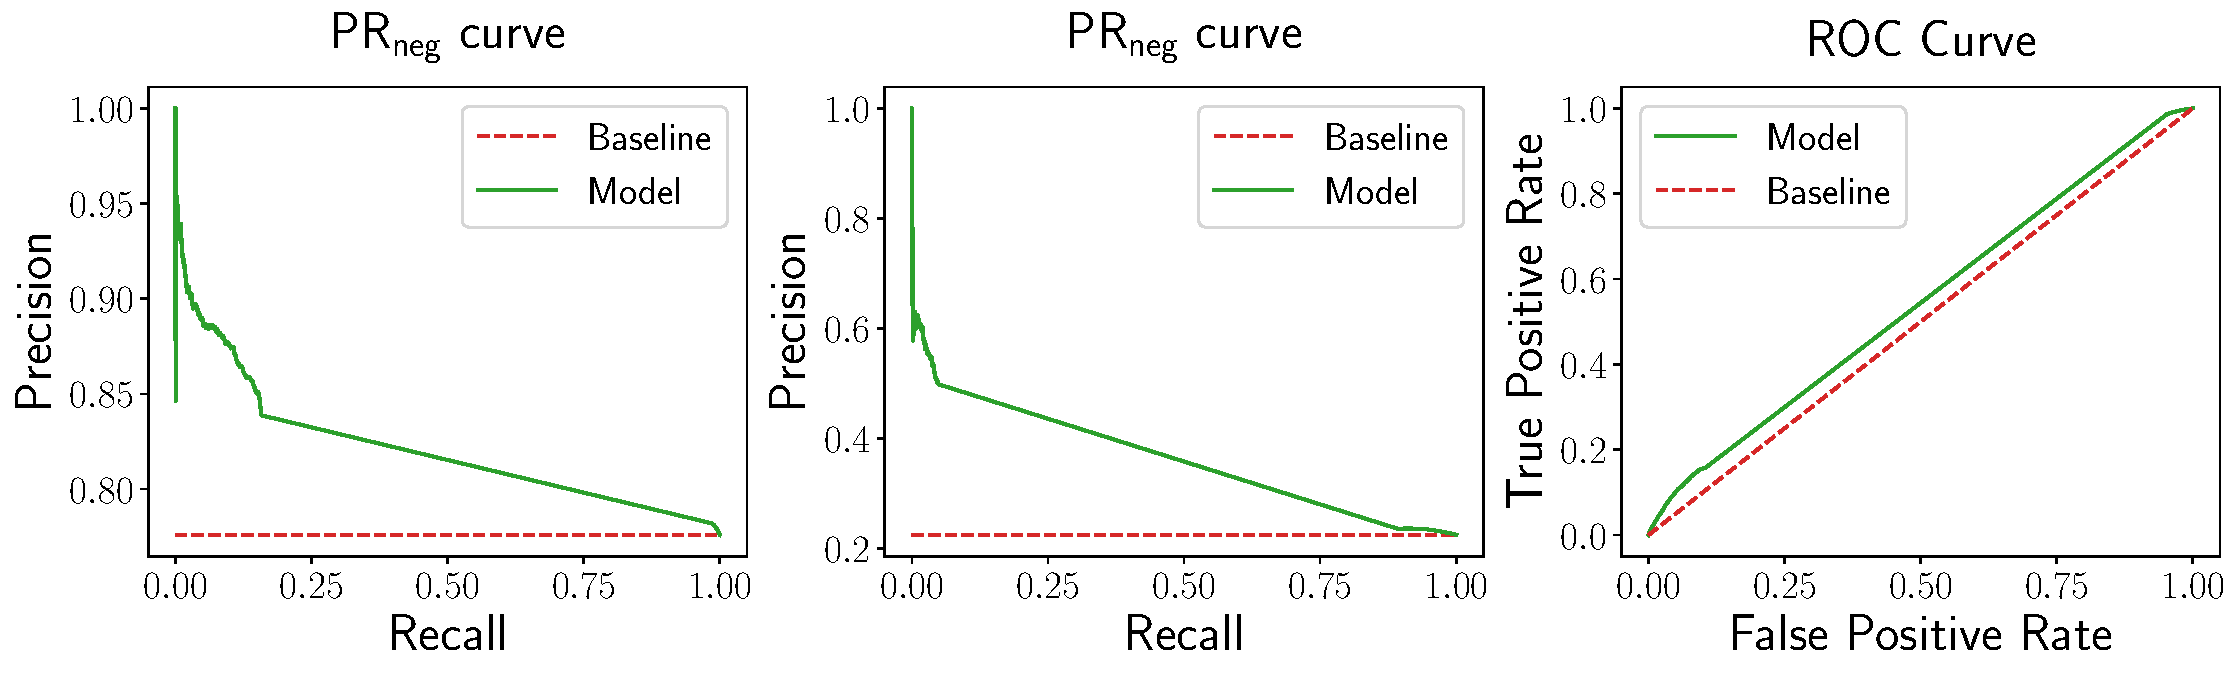
\includegraphics[width=\textwidth]{images/Logisitc Regression_test.pdf}
    \caption{Logistic Regression plots for test data}
    \label{fig:lr-test-plots}
\end{figure}
\begin{itemize}
    \item the description of the auxiliary graphs 
    \item Present results for LR model
    \item Show the ROC and PR curves
    \item Show the feature importances and discuss their relevance 
    \item Highlight the difficulty of predicting negative votes
\end{itemize}

\subsection{Iterative Model Results}
\begin{itemize}
    \item discuss how to compare the iterative model results
    \item Provide plots and table 
    \item Discuss the predictive power of the iterative model over the combination model
    \item Limitations and expansion of the graph combination model
\end{itemize}

\section{Complete \wikirfa Results}
\label{sec:complete-reults}
\begin{table}[htp]
    \centering
    \caption{Results of iterative models on the complete \wikirfa dataset}
    \label{tab:complete-results}
    \begin{tabular}{lccc}
        \toprule
        Model & AUC-ROC & \aucposPR  & \aucnegPR \\ 
        \midrule
        
        Baseline & 0.5 & 0.784& 0.216 \\

        Iterative Balance &  0.835 & 0.935 & 0.635 \\

        Iterative Status & 0.784 & 0.917 & 0.502 \\
        
        \bottomrule
        \end{tabular}
\end{table}

\begin{figure}[htp]
    \centering
    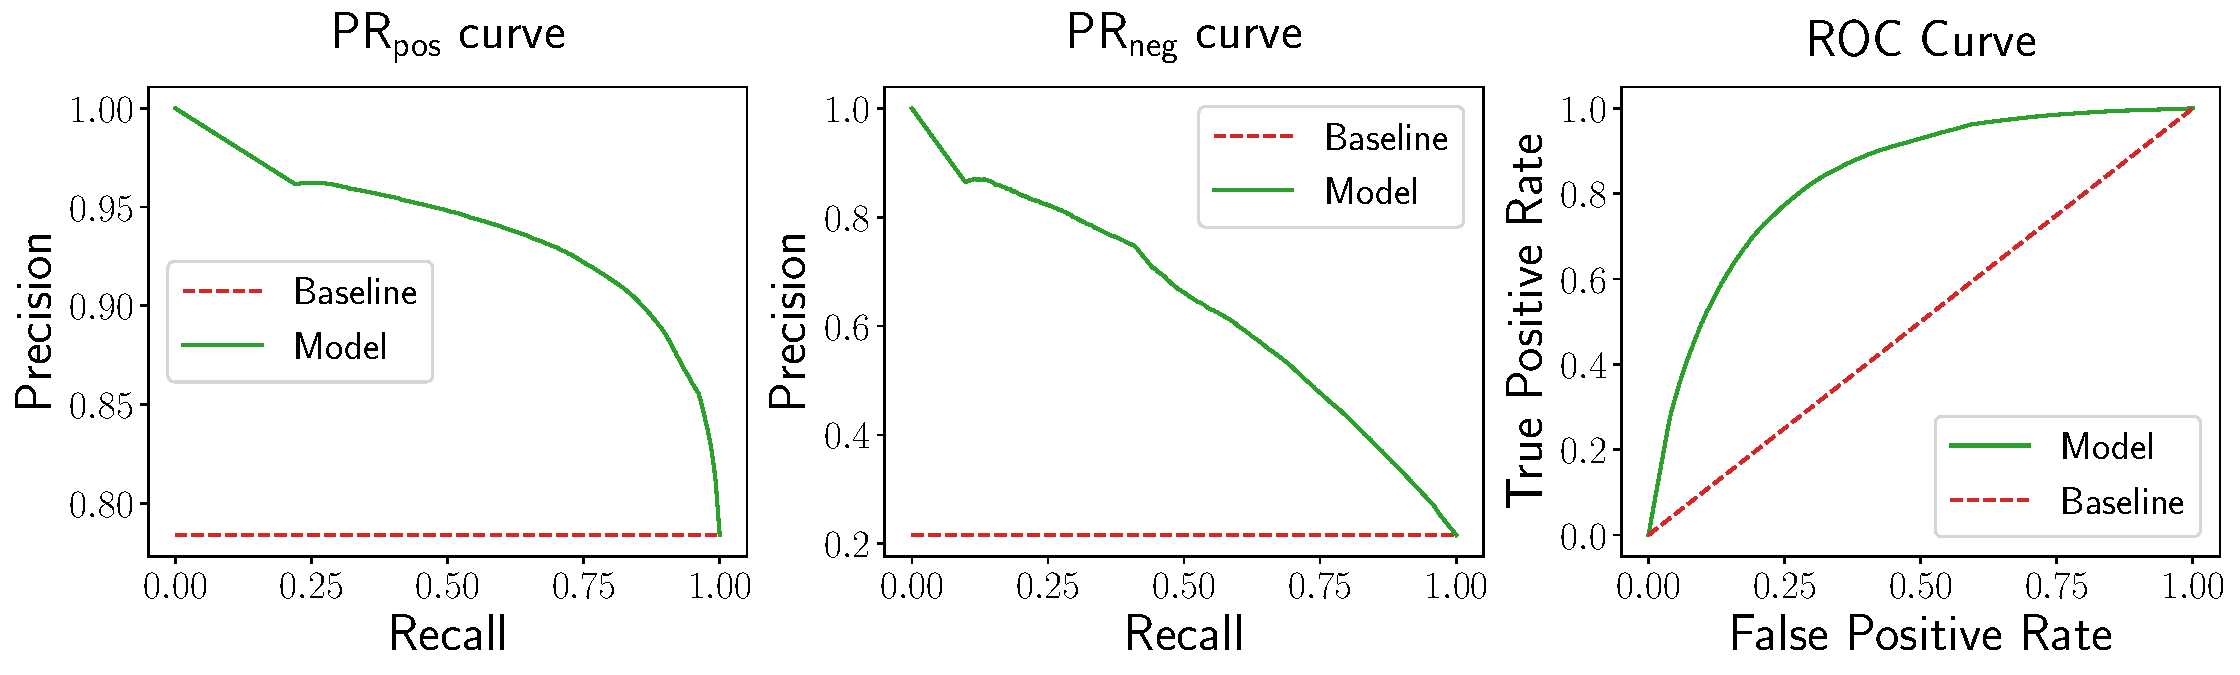
\includegraphics[width=\textwidth]{images/iterative_Balance.pdf}
    \caption{Plots for the Iterative Balance Model on the complete \wikirfa dataset}
    \label{fig:complete-iterative-balance}
\end{figure}

\begin{figure}[htp]
    \centering
    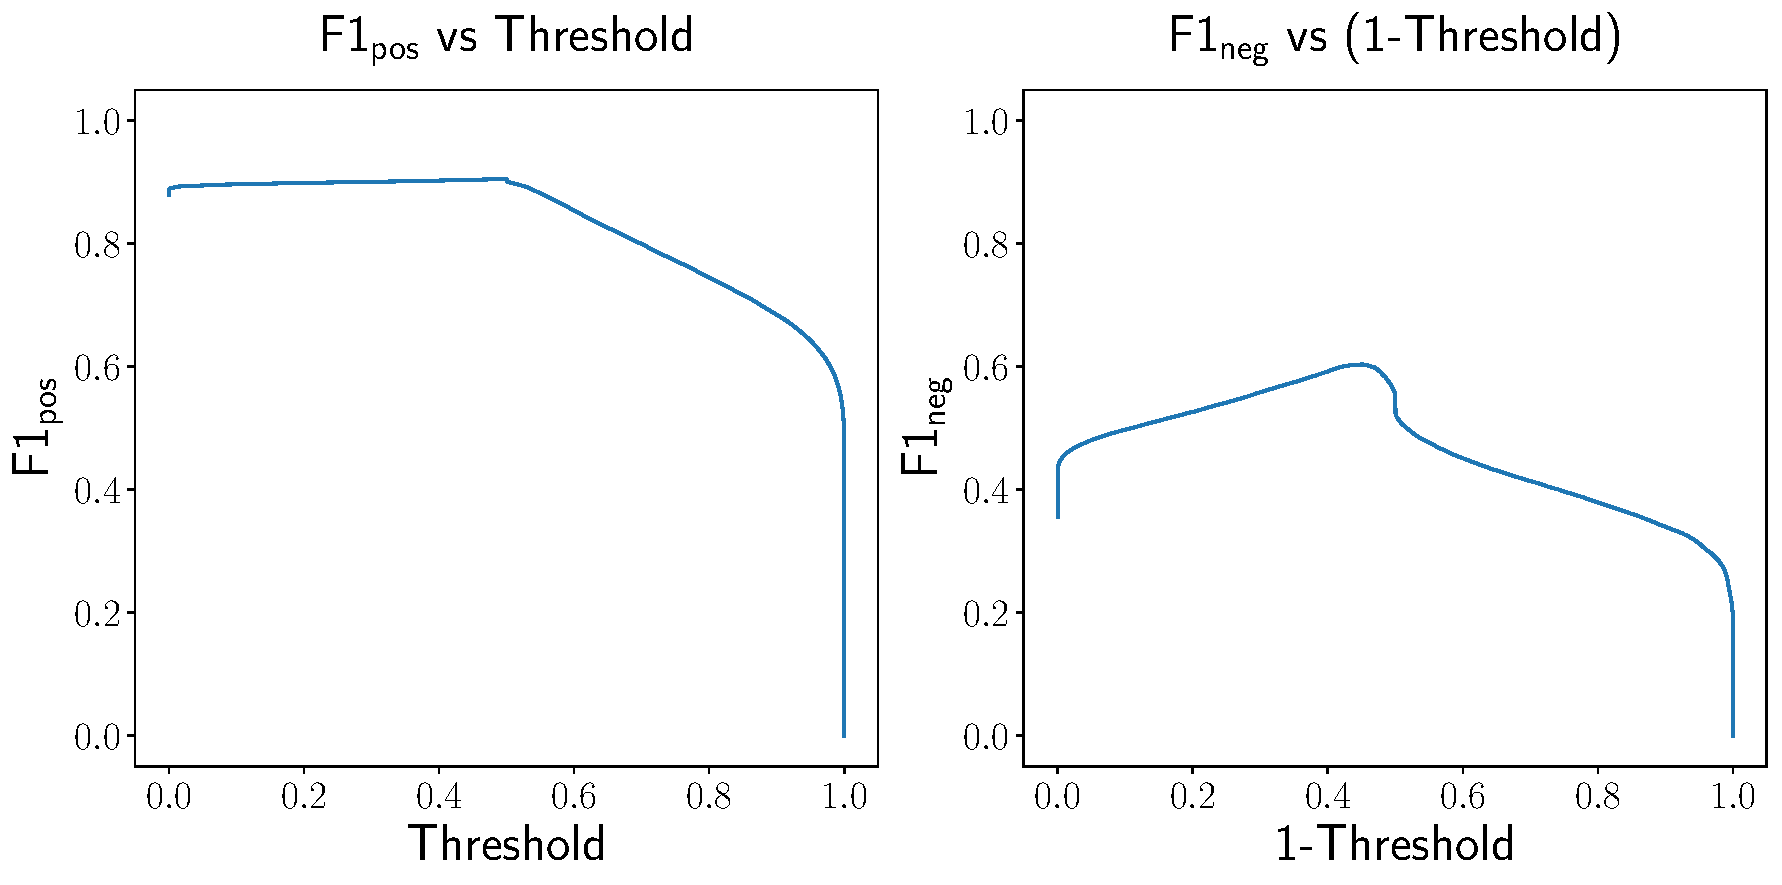
\includegraphics[width=0.75\textwidth]{images/iterative_Balance_f1.pdf}
    \caption{F1 score versus threshold plots for Iterative Balance Model}
    \label{fig:complete-iterative-balance-f1}
\end{figure}


\begin{figure}[htp]
    \centering
    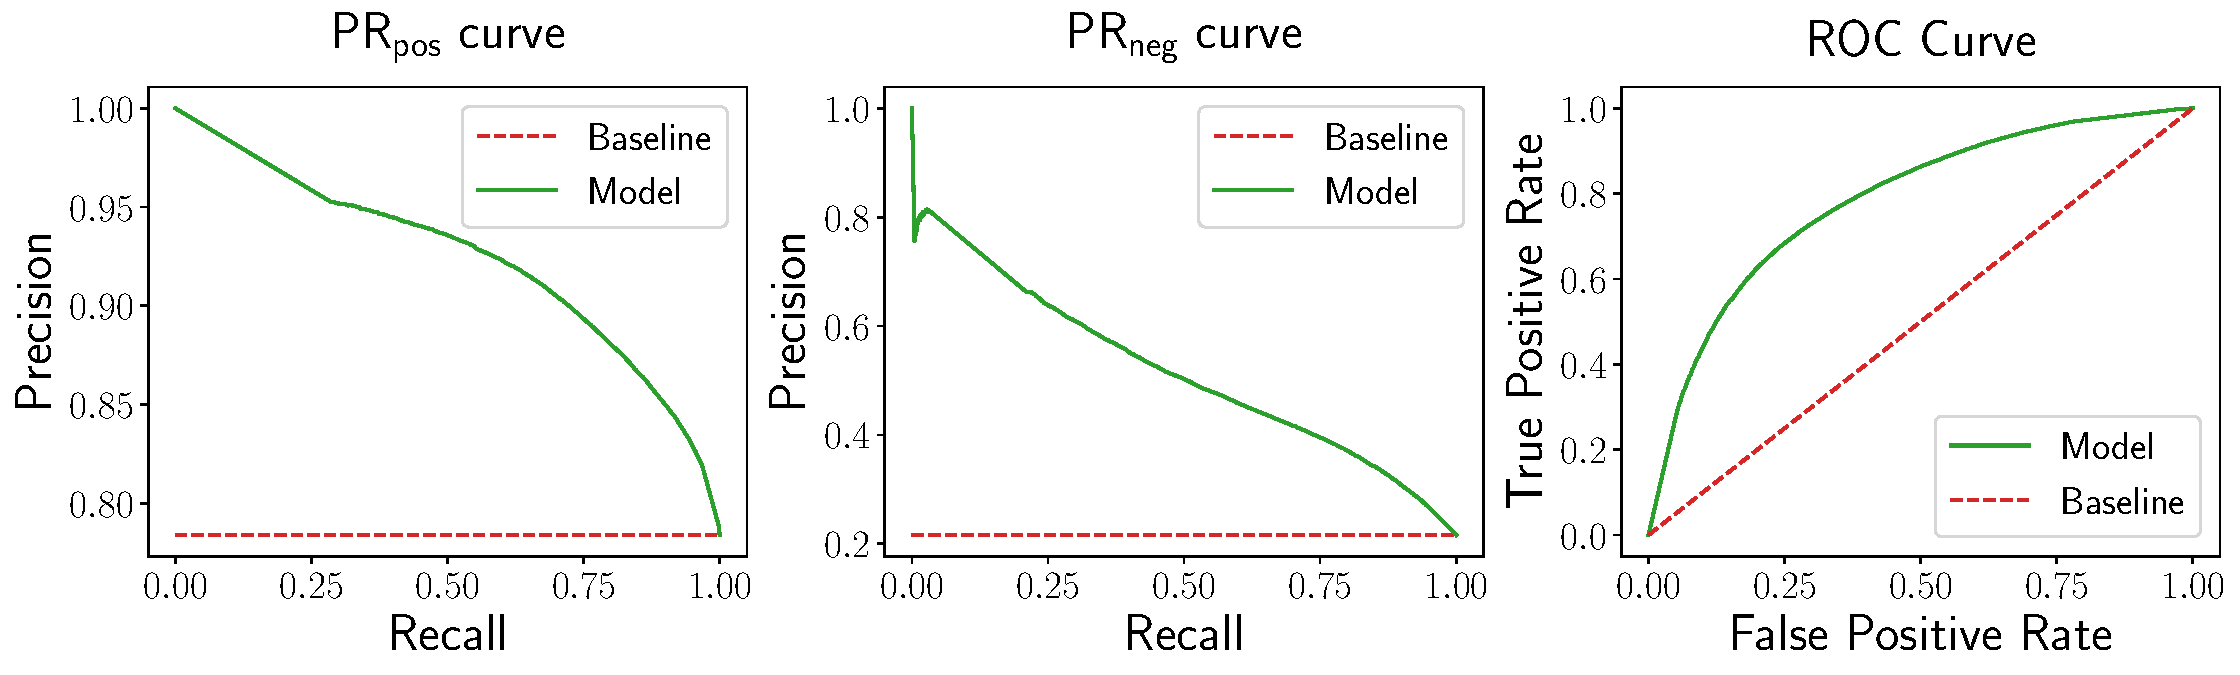
\includegraphics[width=\textwidth]{images/iterative_Status.pdf}
    \caption{Plots for the Iterative Status Model on the complete \wikirfa dataset}
    \label{fig:complete-iterative-status}
\end{figure}


\begin{figure}[htp]
    \centering
    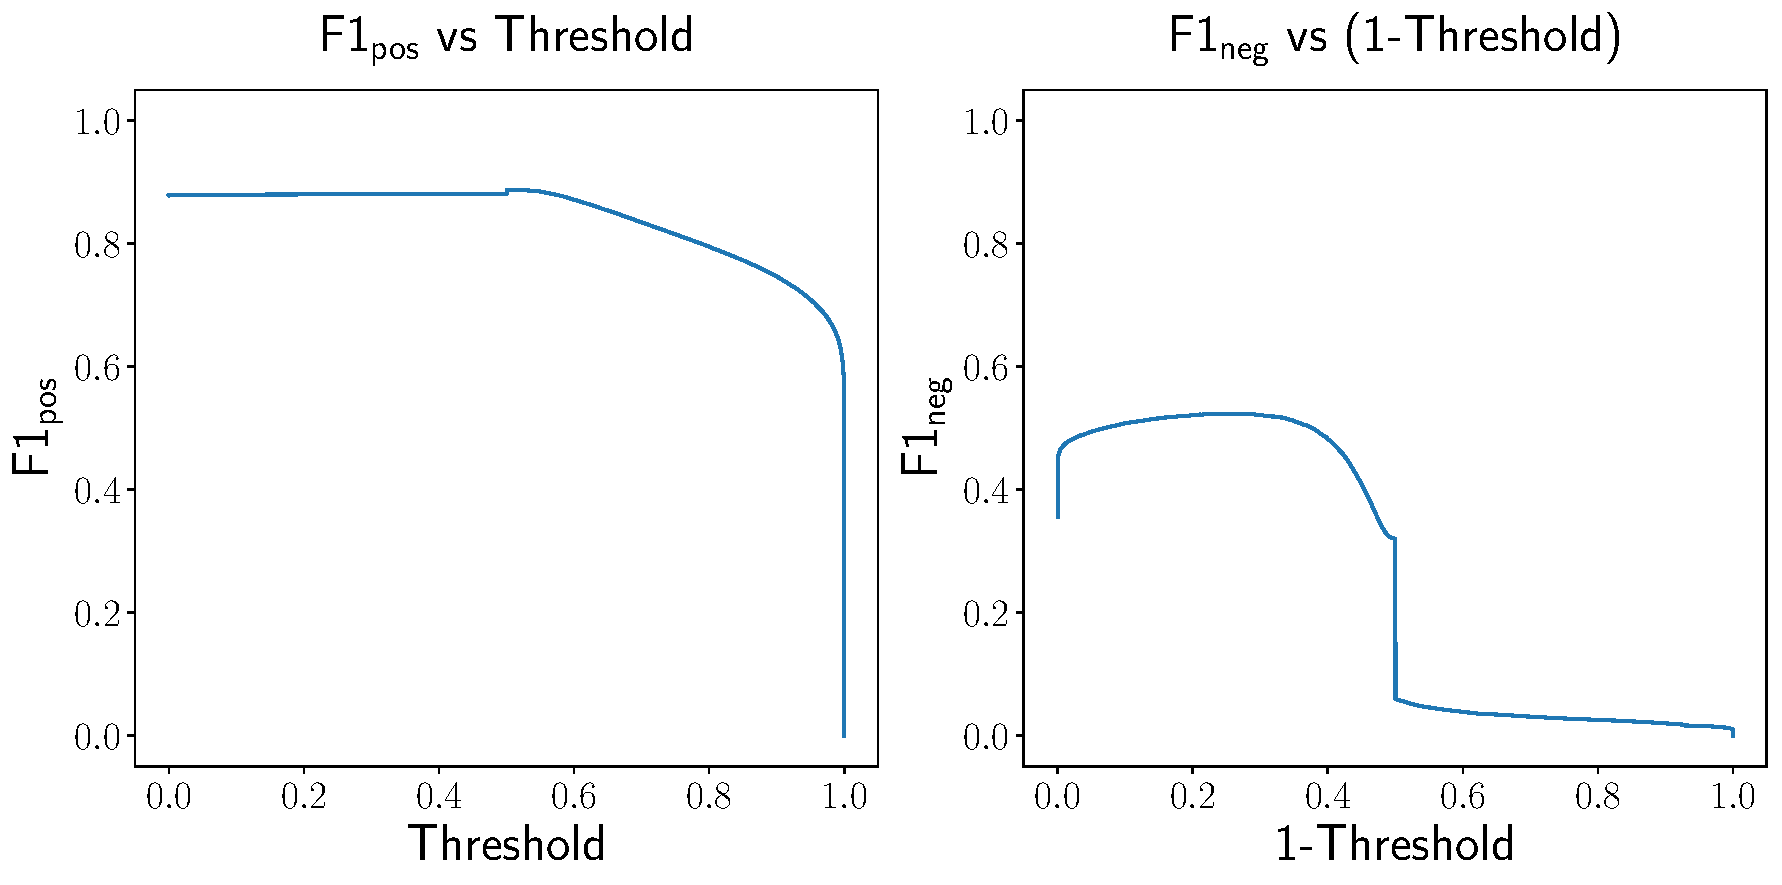
\includegraphics[width=0.75\textwidth]{images/iterative_Status_f1.pdf}
    \caption{F1 score versus threshold plots for Iterative Status Model}
    \label{fig:complete-iterative-status-f1}
\end{figure}



\begin{itemize}
    \item Present the Iterative Balance model results
    \item Discuss quality of predictions using evaluation metrics
    \item Explain the Iterative Status model results 
    \item Explain the selection of threshold and F1-score
\end{itemize}

\section{Voting Order Results}
\label{sec:voting-order-results}
\begin{table}[htp]
    \centering
    \caption{Results for different vote orderings for the failed RfA}
    \label{tab:fail-rfa}
    \begin{tabular}{llccc}
        \toprule
        Model & Vote Order & AUC-ROC & \aucposPR  & \aucnegPR \\ 
        \midrule
        
        Baseline & - & 0.5 & 0.52 & 0.479 \\
        \midrule
        
        \multirow{3}{*}{\shortstack[l]{Iterative\\ Balance}} & 
        Normal &  0.543 & 0.74 & 0.454 \\
        % \cmidrule{2-5}
        &Reversed & 0.74 & 0.868 & 0.572 \\
        % \cmidrule{2-5}
        & Random & 0.68 & 0.812 & 0.575 \\
        \midrule

        \multirow{3}{*}{\shortstack[l]{Iterative\\ Status}} & 
        Normal & 0.962 & 0.977 & 0.909 \\
        % \cmidrule{2-5}
        & Reversed & 0.930 & 0.965 & 0.806   \\
        % \cmidrule{2-5}
        & Random & 0.924 & 0.957 & 0.818 \\
        \bottomrule
        \end{tabular}
\end{table}

\begin{table}[htp]
    \centering
    \caption{Results for different vote orderings for the successful RfA}
    \label{tab:pass-rfa}
    \begin{tabular}{llccc}
        \toprule
        Model & Vote Order & ROC AUC & PR Positive  & Pr Negative \\ \midrule
        Baseline & - & 0.5 & 0.905 & 0.095 \\
        \midrule
        
        \multirow{3}{*}{\shortstack[l]{Iterative\\ Balance}} & 
        Normal &  0.9175 & 0.991 & 0.385 \\
        % \cmidrule{2-5}
        &Reversed & 0.720 & 0.972 & 0.142 \\
        % \cmidrule{2-5}
        & Random & 0.894 & 0.989 & 0.431 \\
        \midrule
        
        \multirow{3}{*}{\shortstack[l]{Iterative\\ Status}} & 
        Normal & 0.846 & 0.981 & 0.293 \\
        % \cmidrule{2-5}
        & Reversed & 0.895 & 0.99 & 0.29 \\
        % \cmidrule{2-5}
        & Random & 0.931 & 0.992 & 0.451 \\
        \bottomrule
        \end{tabular}
\end{table}


